% This is a sample document using the University of Minnesota, Morris, Computer Science
% Senior Seminar modification of the ACM sig-alternate style. Much of this content is taken
% directly from the ACM sample document illustrating the use of the sig-alternate class. Certain
% parts that we never use have been removed to simplify the example, and a few additional
% components have been added.

% See https://github.com/UMM-CSci/Senior_seminar_templates for more info and to make
% suggestions and corrections.

\documentclass{sig-alternate}
\usepackage{color}
\usepackage[colorinlistoftodos]{todonotes}

%%%%% Uncomment the following line and comment out the previous one
%%%%% to remove all comments
%%%%% NOTE: comments still occupy a line even if invisible;
%%%%% Don't write them as a separate paragraph
%\newcommand{\mycomment}[1]{}

\begin{document}

% --- Author Metadata here ---
%%% REMEMBER TO CHANGE THE SEMESTER AND YEAR
\conferenceinfo{UMM CSci Senior Seminar Conference, December 2014}{Morris, MN}

\title{Automatic Chord Recognition from Audio}

\numberofauthors{1}

\author{
% The command \alignauthor (no curly braces needed) should
% precede each author name, affiliation/snail-mail address and
% e-mail address. Additionally, tag each line of
% affiliation/address with \affaddr, and tag the
% e-mail address with \email.
\alignauthor
Alex R. Emmons\\
	\affaddr{Division of Science and Mathematics}\\
	\affaddr{University of Minnesota, Morris}\\
	\affaddr{Morris, Minnesota, USA 56267}\\
	\email{emmon046@morris.umn.edu}
}

\maketitle
\begin{abstract}
Automatic chord recognition from audio is used in the area of \textit{Music Information Retrieval} (MIR) to document and categorize music. In addition to providing harmony to music, chords also provide a way to describe the harmony of a piece. In almost every chord recognition system the audio signal is represented by a \textit{Pitch Class Profile} (PCP), which measures the intensity of energy in each of the frequency regions where musical notes occur \cite{Morman:2006}. Some systems perform what is known as preprocessing before generating a PCP, to get rid of unwanted frequencies in the audio file. The next step, known as pattern matching, is to assign chord labels by matching the harmonic features to a set of chord models. In this paper we will discuss these processes in greater detail and compare the results of three research cases, each of which uses a different chord recognition system.
\end{abstract}

\keywords{Automatic chord recognition, hidden Markov models, pitch class profile, signal processing}

\section{Introduction}
A chord is a set of tones played simultaneously. A chord progression is a sequence of chords over time and is what describes the harmony of a piece \cite{Lee:2006}. Automatic chord recognition is the process of extracting a chord progression from an audio file. These chord sequences are used by musicians as lead sheets (summaries containing chords, melody, and lyrics) as well as by researchers for tasks such as key detection, genre classification, and lyric interpretation. Performing chord analysis by hand is time consuming, prone to human error, and requires two or more trained experts. This is what makes automatic chord recognition an important area of research \cite{McVicar:2014}.

The two main steps of automatic chord recognition are feature extraction and pattern matching. Feature extraction is the process of extracting useful information from audio files, and pattern matching is how chord labels are applied to that data. 
%An overview of the system can be seen in Figure~\ref{fig:fig2}.

There are many challenges encountered by systems that process audio signals. There are background noises, percussion instruments, and other unwanted tones in audio recordings. It is also difficult to distinguish when chords change and to line these points up exactly with the beat. Preprocessing helps eliminate unwanted information from the audio files before or during the feature extraction step, depending on the system. An overview of one of the chord recognition systems looked at in this paper can be seen in Figure~\ref{fig:fig2}.

Chord recognition systems have been improving and becoming more usable in recent years. This paper will compare three different systems that use a variety of techniques in each step of the process. By looking at the components of the highest performing systems, we will determine the most effective methods used for each step of the process. 

\begin{figure*}
\centering
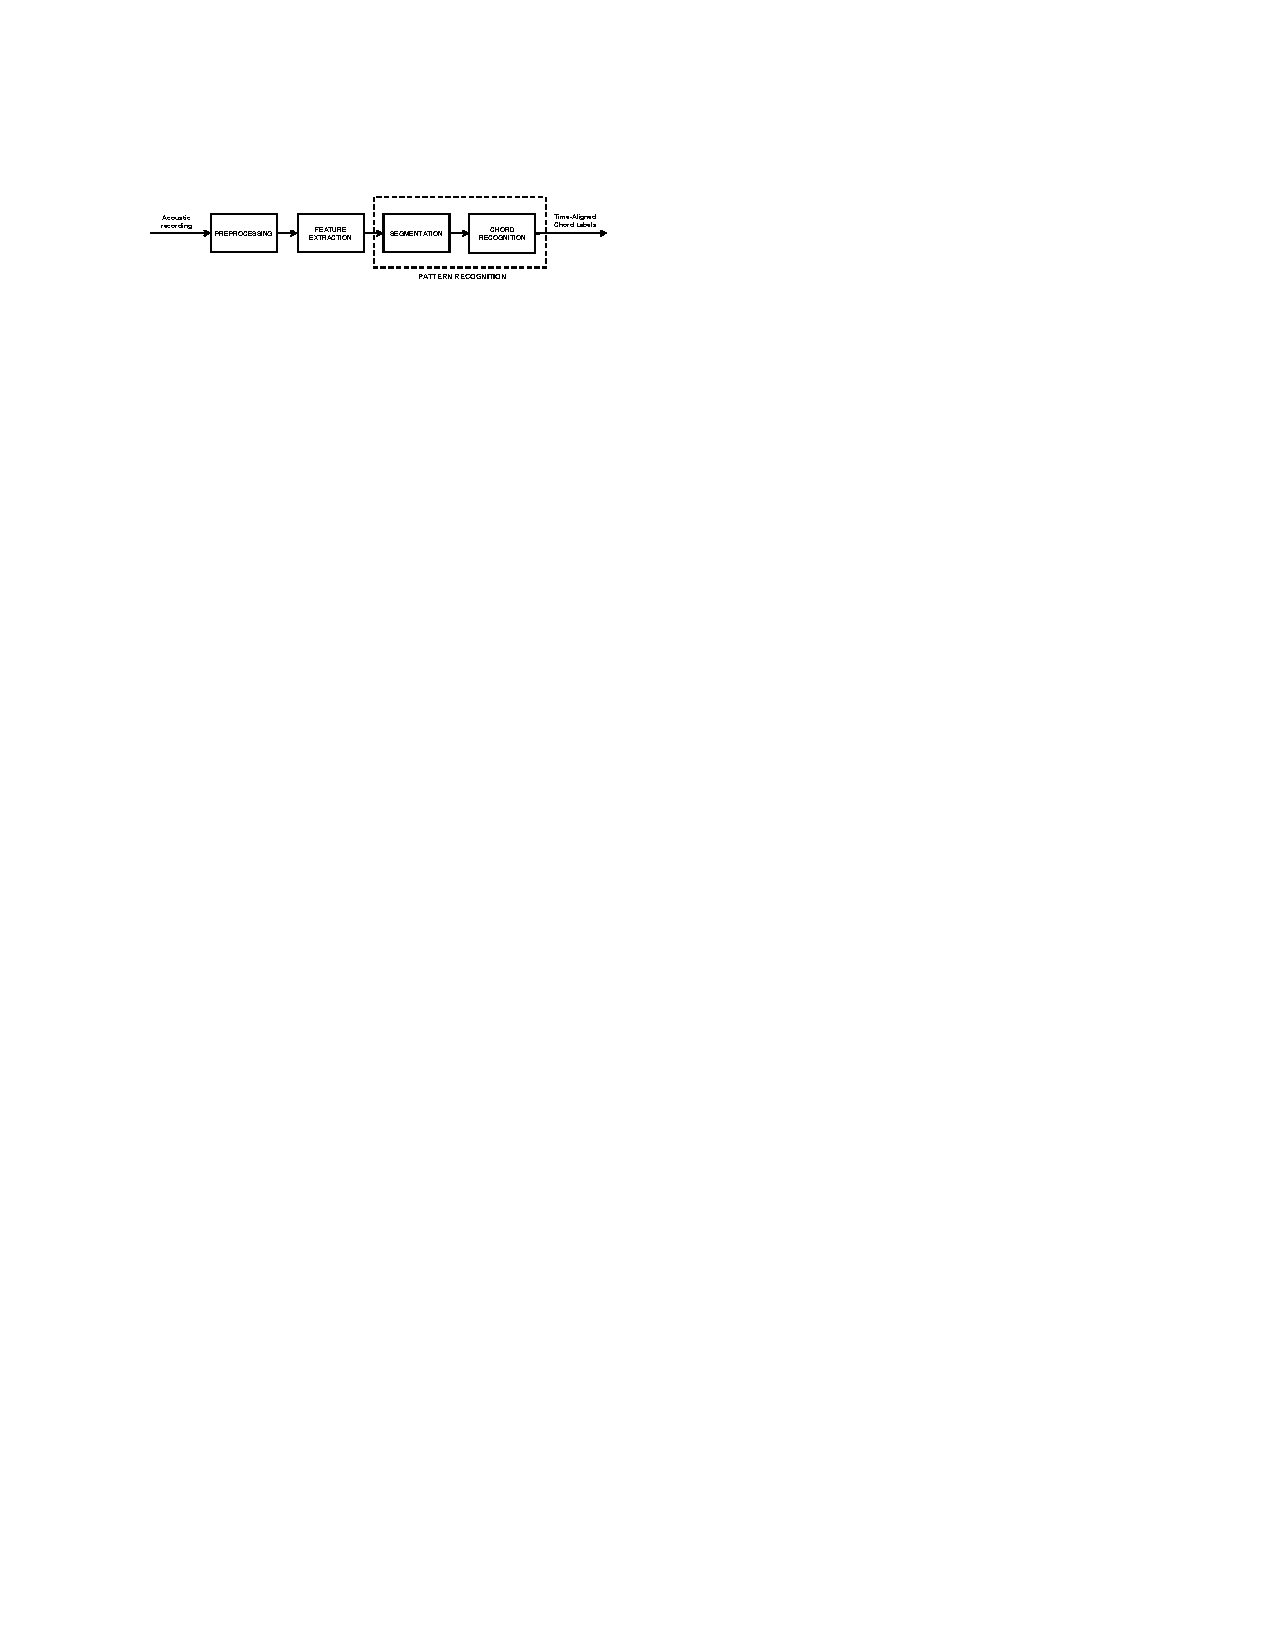
\psfig{file=fig2.pdf,width =5.3in}
\caption{Overview of the chord recognition system used in~\cite{Morman:2006}.}
\label{fig:fig2}
\end{figure*}  

\section{Background}
In order to explain the process of automatic chord recognition, some general information about feature extraction and pattern matching is needed.

\subsection{Feature Extraction}

The first step of generating a chord progression from audio data is processing the signal to extract harmonic features. Feature extraction is a fairly simple process, but can be made more complex by introducing optimization steps to increase accuracy \cite{McVicar:2014}. Preprocessing is one of these steps, performed before calculating \textit{Pitch Class Profile} (PCP), which is a representation what notes are present over time.

\subsubsection{Preprocessing}

In Figure~\ref{fig:fig4} the light areas show where frequencies have been detected, and the dark areas show empty space. It is clear that frequencies other than just the chord tones have been detected because the light areas are not solid white and the dark areas not solid black. The goal of preprocessing is to reduce as much of this background noise as possible from the audio file, in an effort to provide a smooth and clear PCP. Depending on the audio resolution, very low pitches can be hard to distinguish and tend to blur across multiple pitches. Percussion sounds also need to be addressed, especially those that create a pitch such as a bass drum.

Another issue is that musical instruments produce a series of harmonics at higher and lower frequencies than the tone that is played. These tones, called overtones, can confuse feature extraction techniques and need to be removed.

%Preprocessing and pre-/post-filtering are optional steps but all of the systems in this paper use it in some way. The reason is that audio files are not perfect; they contain other tones and frequencies that are unrelated to the chords being played. Musical instruments also produce what are known as overtones, tones that sound above or below the note that was played \cite{TaeMin:2014}. Preprocessing is done to the raw audio file, to remove unwanted noise and frequencies. Pre-filtering is done after the feature extraction step, in order to smooth out the PCP. Post-filtering is done after the chords have been determined by the pattern recognition step, finding the most likely sequence and eliminating unlikely chords.

\todo[inline]{Explain two types of preprocessing, background spectrum and overtone removal. Explain types and how they work and give more info. Explain more about overtones and how they are detected, give more examples of 'other tones'. the sum of sinusoidal tones of integer multiples of the fundamental frequency. Add a figure.}

\subsubsection{Pitch Class Profile} 

The pitch of a note is measured in two dimensions - height and chroma (pitch class). Height tells which octave a note belongs to, and chroma tells where a note stands within the octave (the name of the note). Height is not a factor in determining chord type because two notes that are an octave apart have the same chroma value. A chromagram, or PCP, is a 12-dimensional vector representation of chroma, representing the intensity of each of the twelve semitones in the chromatic scale, over a period of time. An example of a common PCP, along with the actual progression, can be seen in Figure~\ref{fig:fig4}~\cite{McVicar:2014}. For over a decade PCP has been the most popular way to represent harmonic features for chord recognition. Most new approaches are variations or refinements of this approach \cite{TaeMin:2014}. Modern systems can have many more steps in converting audio to PCP including tuning correction, which compensates for music that is not tuned to standard pitch \textit{A4 = 440 Hz}, and beat-synchronization, which calculates the average pitch between beats to get rid of changes caused by noise and other transients. \cite{McVicar:2014}.

\todo[inline]{Describe them or some of them. Decide between using pitch class and chroma. More detail in paper 1 under feature extraction}

\begin{figure}
\centering
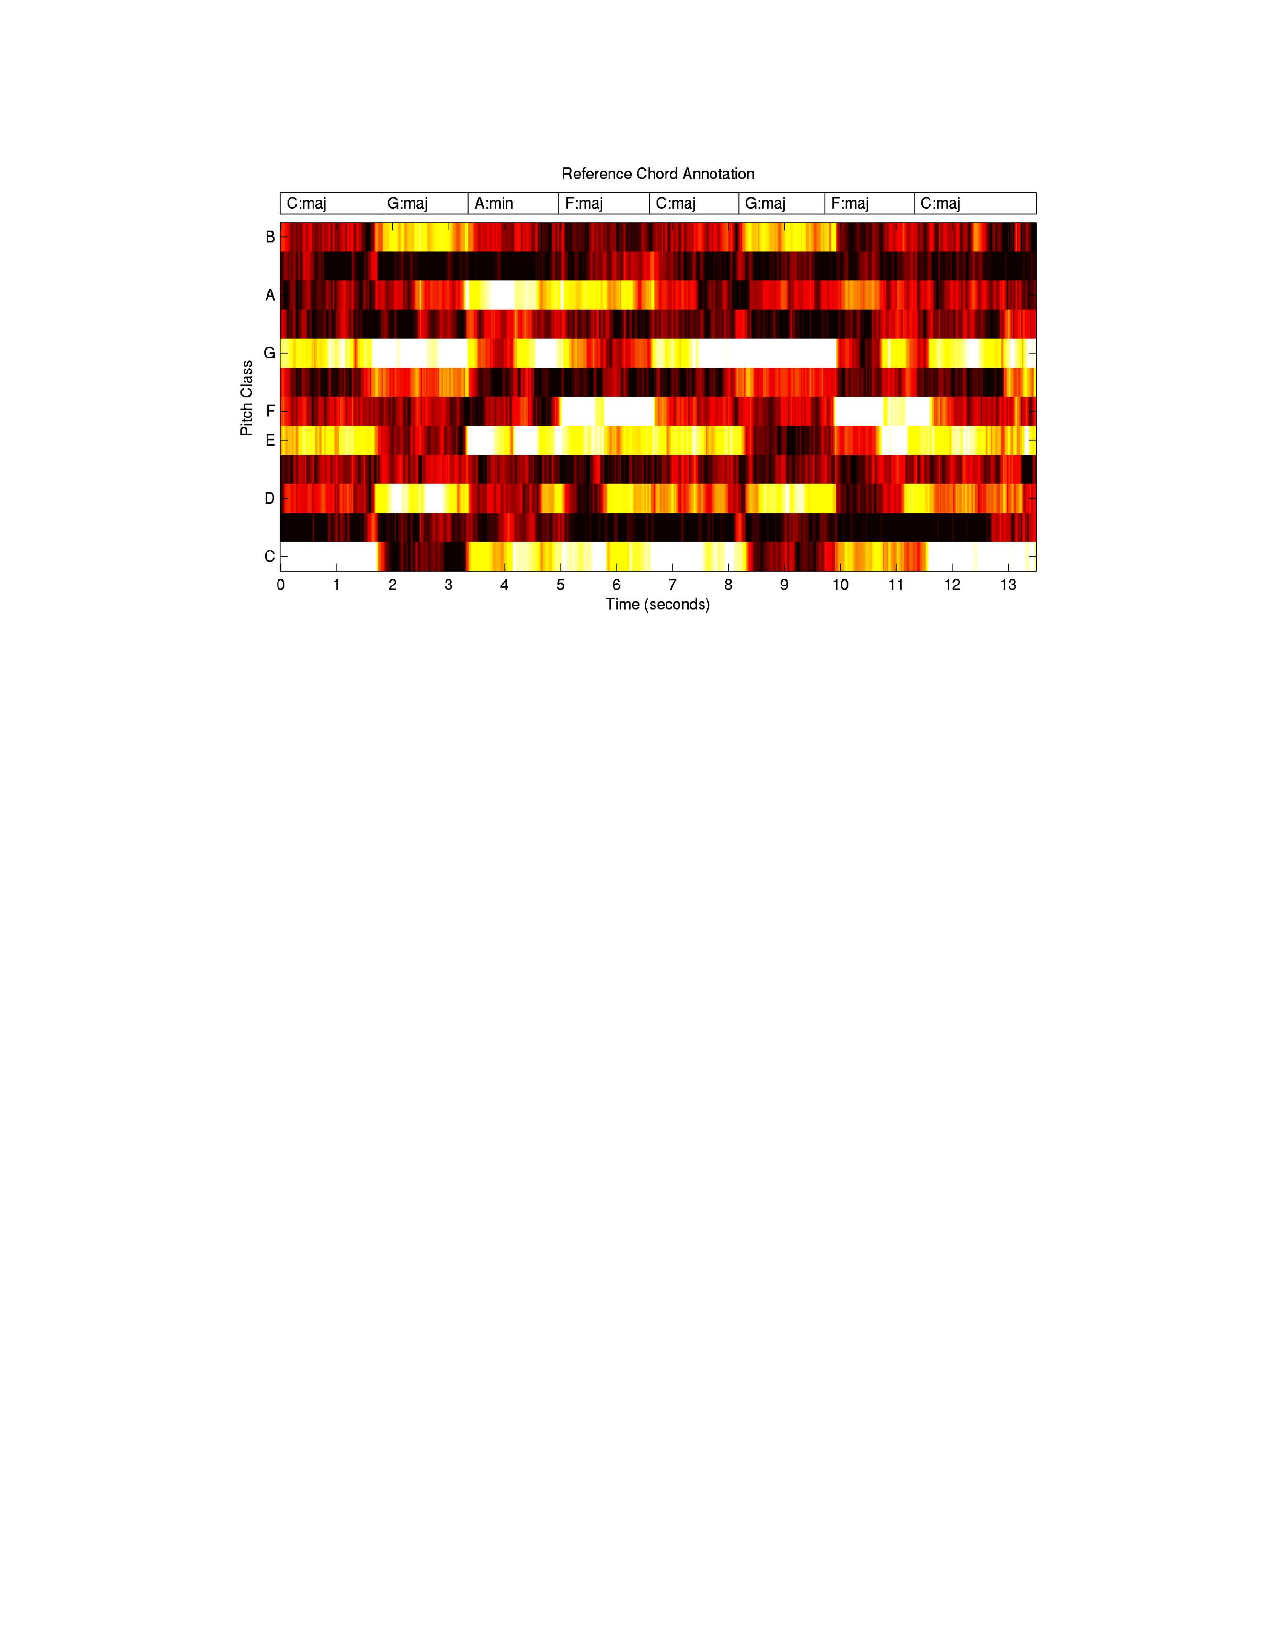
\psfig{file=fig4.pdf,width =3in}
\caption{A typical chromagram, or PCP, generated from the opening to \textit{Let It Be} (Lennon/McCartney). Pitch class (chroma) at time t is shown by the intensity or lightness at that point. The true chord progression (simplified) is shown above for comparison.}
\label{fig:fig4}
\end{figure}


\subsection{Pattern Matching}

\todo[inline]{Decide between pattern recognition and pattern matching.}

Almost all chord recognition systems use PCP or some other chroma-based feature extraction technique. What differentiates these systems is the mechanism used to label chords.\todo[inline]{Define chord model.} Generating the chord model against which the PCP will be matched can be done in one of two ways: manually using musical knowledge, or stochastically, by deriving it from real-world music. In a manual system the chroma values being sounded are compared against pre-defined chord templates.\todo[inline]{Define these better.} These two methods are compared by Cho and Bello in  \cite{TaeMin:2014}. Stochastic chord models are more sophisticated and complex. HMMs used to be the method of choice, but many recent systems prefer Gaussian mixture models \cite{TaeMin:2014}.

\todo[inline]{Add sentance describing stocastic chord model system after manual system. Get rid of more sophisticated and complex.}

\subsubsection{Hidden Markov Models}\label{main} 

A \textit{hidden Markov model} (HMM) is a statistical model which describes a finite set of states, in this case chords, each with a probability distribution. Transitions between these states are governed by a set of transition probabilities that describe the likelihood of transitioning from one to another \cite{TaeMin:2014}. HMMs are used in a wide variety of pattern recognition environments such as speech, handwriting, and gesture recognition, as well as in bioinformatics. 

\todo[inline]{Need to re-write this section from draft. Include figures for models. find first instance of HMM.}

\subsubsection{Gaussian Mixture Models}

\textit{Gaussian mixture models} (GMMs) are used in many modern chord recognition systems. A GMM consists of a distribution of weighted Gaussian components that represent descriptions of each chord in the training data.\todo[inline]{Need a better definition} To train these models the PCP from the training data is transposed to all C-based chords (C-major and C-minor). These normalized chords are used to train the C-major and C-minor models, and then re-transposed to the remaining 11 keys~\cite{TaeMin:2014}.

\todo[inline]{Need more here. REWRITE}

\subsubsection{Support Vector Models}

\section{Research Cases}

This paper looks at three research cases that involve automatic chord recognition. All of the cases use three common steps in the process: feature extraction, preprocessing, and pattern recognition. Here we will give an overview of each system and the datasets that were used.

\todo[inline]{Decide between study and case.}

\subsection{Case 1: Effects of Proper Signal Processing}

The first study~\cite{Morman:2006} uses a chord recognition system that begins with a preprocessing block, followed by feature extraction, where PCP is calculated. After this, the signal is segmented along predicted chord boundaries, and then chord labels are assigned to each segment. An overview of this system can been seen in Figure~\ref{fig:fig2}~\cite{Morman:2006}. 

There are two stages in the preprocessing block, to address background noise and overtones. The first step, Homomorphic Liftering, is a method of separating out the frequencies of musical tones from background and system noise. This is done by finding strong frequency peaks in areas corresponding to the pitch range of the notes. Frequencies above and below a specified range can also be removed to reduce noise. The second step, known as the \textit{Harmonic Product Spectrum} (HPS), is a method which emphasizes frequencies when their overtones are present. HPS is calculated by compressing the spectrum by factors of 1 to R and multiplying the resulting compressed spectra. The resulting output energy is then summed according to pitch class and a PCP is created.

The first step of pattern matching for this system is chord segmentation, where the audio signal is segmented at the boundaries where chords change. This can be difficult because some chords are not played all at once, the notes are played in sequence and held. To find the points where change has occurred the PCP is analyzed frame-by-frame to find significant change in pitch-class content. 

The next and final step is assigning chord labels to the segments. Given an instance of the PCP for a region of the audio, the most probable chord label is picked from a set of training PCPs. In this study the use of GMMs and SVMs is compared.

\subsubsection{Datasets}

In this experiment \textit{MIDI} (Musical Instrument Digital Interface) recordings were used to create time aligned labelled audio. Two datasets were used: one of isolated chords synthesized on piano and strings, and one of continuous single-instrument audio synthesized on piano. 

The isolated chord dataset consisted of 7790 chords and inversions, where the notes are stacked in a different order. Three chord complexity levels were tested, labelled DS1, DS2, and DS3. The first involved the common triad types (major, minor, augmented, and diminished), the second included variations of the 7th chord (major 7th, minor 7th, dominant 7th, fully diminished 7th, and half diminished 7th), and in the third all 11 different chord types that the system could recognize were used.\todo[inline]{Need to somehow name these and reference them as DS1,2,3 in table.} This can be seen in Table~\ref{tab:tab1}. Four feature vectors (FV), or models were used for comparison on each of these datasets, which can be seen in Table~\ref{tab:tab2}. The first model started with preprocessing using homomorphic liftering and harmonic product spectrum. FV2 has a low sampling rate and no preprocessing, FV3 increases the sample rate and FFT length, and FV4 first preprocessed the signal and then used the same homomorphic processing and HPS as FV1.

\todo[inline]{Need more info here. Decide between using FV and model. Define liftering HPS and alot of other things. Explain table 2 and use the same terminology here.}

The continuous single-instrument audio dataset consisted of 50 hymn verses selected from the Trinity Hymnal, with 40 used for training and 10 used for testing. FV4 was used from the isolated chord experiment \cite{Morman:2006}. 

%In the experiments two pattern recognition methods are compared: GMMs and Support Vector Machines (SVM). For SVM classification, the OSU SVM Classifier MATLAB Toolbox was used. 

\todo[inline]{Explain SVM in a separate section or leave out.}

\begin{table}
\centering
\begin{tabular}{|c|c|c|c|} \hline
&\multicolumn{3}{|c|}{Label used in:} \\ \hline
Chord Label & DS1A & DS1B & DS1C \\ \hline
Major & Major & Major & Major \\ \hline
Minor & Minor & Minor & Minor \\ \hline
Major 7 & - & Major & Major 7 \\ \hline
Minor 7 & - & Minor & Minor 7 \\ \hline
Dom. 7 & - & Major & Dom. 7 \\ \hline
Dim. & Dim. & Dim. & Dim. \\ \hline
Full Dim. & - & Dim. & Full Dim. \\ \hline
Half Dim. & - & Dim. & Half Dim. \\ \hline
Augmented & Aug. & Aug. & Augmented \\ \hline
Sus. 4 & - & - & Sus. 4 \\ \hline
7 Sus. 4 & - & - & 7 Sus. 4 \\ \hline
\end{tabular}
\caption{Labels used for isolated chord data.}
\label{tab:tab1}
\end{table} 

\begin{table}
\centering
\begin{tabular}{|c|c|c|c|c|c|} \hline
 & Type & Sampling Rate & FFT Ln. & Lifter & HPS R \\ \hline
FV1 & FB & 44100 & 32768 & yes & 5 \\ \hline
FV2 & PCP & 11025 & 4096 & no & 1 \\ \hline
FV3 & PCP & 44100 & 32768 & no & 1 \\ \hline
FV4 & PCP & 44100 & 32768 & yes & 5 \\ \hline
\end{tabular}
\caption{Feature Vectors used in isolated chord recognition.}
\label{tab:tab2}
\end{table} 

\subsubsection{Results}

For the isolated chords dataset, this system was trained using chords synthesized on a piano, and was tested on chords synthesized on both piano and strings. The dataset was randomly divided with 80\% of the chords used for training and 20\% for testing. Five of these training and testing sets were created and the recognition rates from these were averaged. The overall chord recognition accuracies for piano can be seen in table~\ref{tab:tab3} and for strings in table~\ref{tab:tab4}. FV4 performed the best with the chords played on strings, and showed the least difference between recognizing piano and string chords \cite{Morman:2006}.

For the continuous single-instrument dataset, only FV4 was used.

\todo[inline]{Need to add results of the continuous single-instrument dataset.}

\begin{table}
\centering
\begin{tabular}{|c|c|c|c|} \hline
Feature Vector & DS1A & DS1B & DS1C \\ \hline
FV1 & 83.68 & 61.85 & 57.24 \\ \hline
FV2 & 90.33 & 82.44 & 82.26 \\ \hline
FV3 & 91.76 & 84.20 & 84.09 \\ \hline
FV4 & 85.64 & 79.40 & 78.93 \\ \hline
\end{tabular}
\caption{Isolated chord recognition accuracy using GMM, training set: piano, testing set: piano.}
\label{tab:tab3}
\end{table} 

\begin{table}
\centering
\begin{tabular}{|c|c|c|c|} \hline
Feature Vector & DS1A & DS1B & DS1C \\ \hline
FV1 & 68.06 & 42.00 & 33.62 \\ \hline
FV2 & 42.72 & 18.60 & 16.30 \\ \hline
FV3 & 43.49 & 22.00 & 18.31 \\ \hline
FV4 & 86.94 & 80.23 & 80.18 \\ \hline
\end{tabular}
\caption{Isolated chord recognition accuracy using GMM, training set: piano, testing set: strings.}
\label{tab:tab4}
\end{table}



\subsection{Case 2: HMM with Audio From Symbolic Data}

The next study \cite{Lee:2006} uses a supervised HMM trained with audio from symbolic data.\todo[inline]{Supervised and audio from symbolic data is not defined.} The system used here begins with feature extraction, again using PCP. At the same time, chord label data is generated from the MIDI data that was used to generate the audio. This data is used to train a 36-state HMM \cite{Lee:2006}. These 36 states represent 36 chords - major, minor, and diminished for each 12 notes. The system is trained on a dataset, and then fed a separate dataset for testing and analysis.

\todo[inline]{Need transition here.}

Using an ergodic model, which allows every possible transition from chord to chord, the model parameters are learned, and then the Viterbi algorithm is applied. The Viterbi algorithm finds the most likely path, or chord sequence, by restricting unlikely chord transitions \cite{TaeMin:2014}. Two elements are needed to train this model: chord label files, and audio data. In this case they are both being generated from the same symbolic data. See figure~\ref{fig:fig1} for a representation of this. The first step is to use a chord analysis tool to generate a file with complete chord information for a piece of music. Using the same symbolic data, the audio files are generated using a sample-based synthesizer. This audio data is in perfect sync with the chord label file, and simulates a real recording because it contains the overtones that would be generated from real instruments \cite{Lee:2006}.

\todo[inline]{Need to re-write from section draft! More on Viterbi.}

\begin{figure}
\centering
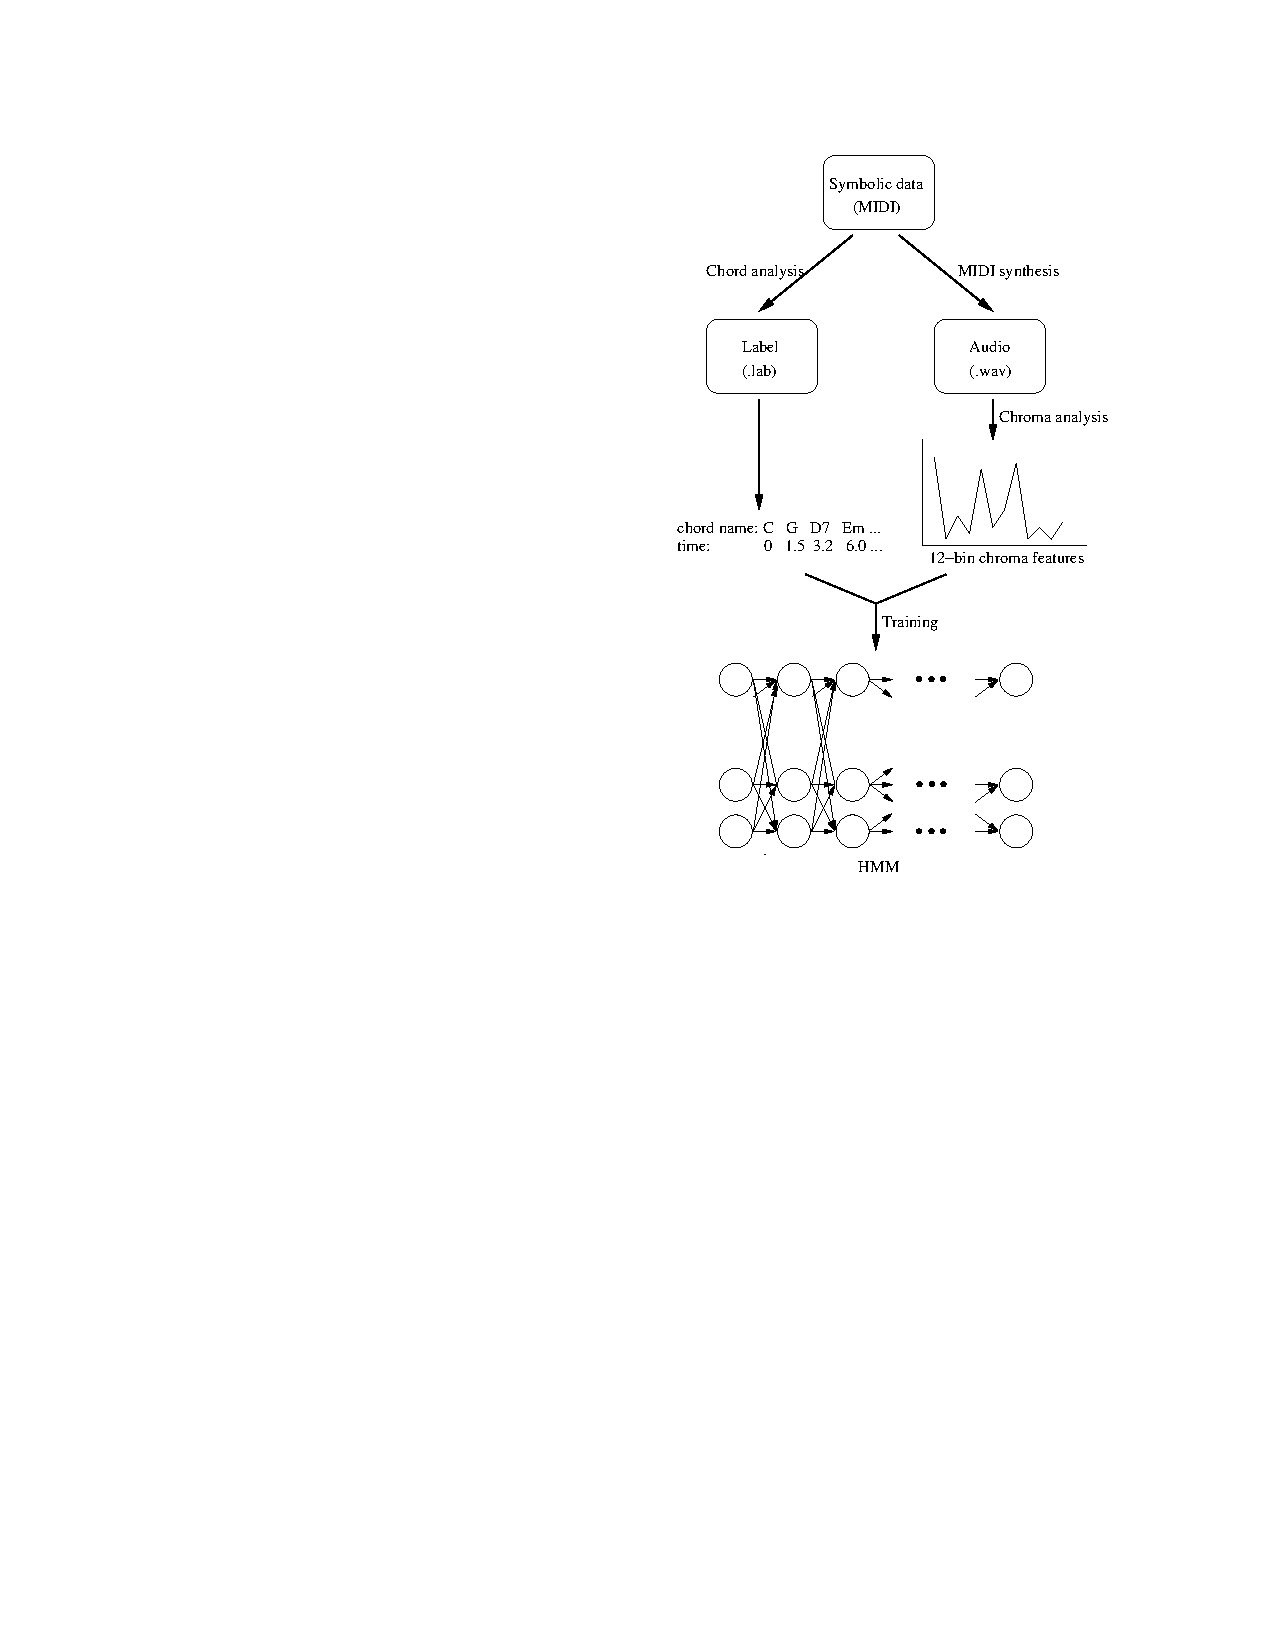
\psfig{file=fig1.pdf,width =3in}
\caption{Overview of the HMM trained with audio from symbolic data in~\cite{Lee:2006}.}
\label{fig:fig1}
\end{figure}

\subsubsection{Datasets}

The training data used for the first model in this case consisted of 81 solo piano pieces by J.S. Bach, Beethoven, and Mozart. For the second case 196 string quartet pieces by Beethoven, Haydn, and Mozart were used. The models were then tested on excerpts from the Kostka and Payne's book, which includes analysis and audio recordings done by the composers. 10 excerpts - 5 piano solos and 5 string quartets were selected, with no overlap of the training data. The output was compared to the hand-marked data for frame rate accuracy \cite{Lee:2006}. 

\subsubsection{Results}

In this case there are two datasets, piano and strings, and each can be tested on a system that is trained with either piano or strings. So each combination was tested, in addition to testing on a system trained with both piano and strings. The results of these experiments can be seen in table~\ref{tab:tab5}.

\begin{table}
\centering
\begin{tabular}{|c|c|c|} \hline
Training Data & Test Data & Recognition Rate \\ \hline
Piano & Piano & 68.69 \\ \hline
String Quartet & Piano & 73.40 \\ \hline
All & Piano & 74.41 \\ \hline
Piano & String Quartet & 79.35 \\ \hline
String Quartet & String Quartet & 79.76 \\ \hline
All & String Quartet & 80.16 \\ \hline
\end{tabular}
\caption{Recognition results for HMM trained with audio from symbolic data.}
\label{tab:tab5}
\end{table}

\subsection{Case 3: Importance of Individual Components}

The final study \cite{TaeMin:2014} compares the most common methods of each step: feature extraction, pattern recognition, and pre/post filtering. This study describes the overall system a little differently than the other two, with preprocessing included in the feature extraction stage, and HMMs included in the post-filtering stage. The pre-filtering stage is where attempts are made to smooth out the PCP. 

Four experiments were conducted in this study: Feature extraction and pattern matching, effect of pre-filtering, effect of post-filtering, and combined pre- and post-filtering. Each experiment was run on 495 chord annotated pop songs. An overview of the system can been seen in figure~\ref{fig:fig3}.

\todo[inline]{decide between chord-annotated and hand marked or define difference.}

\begin{figure}
\centering
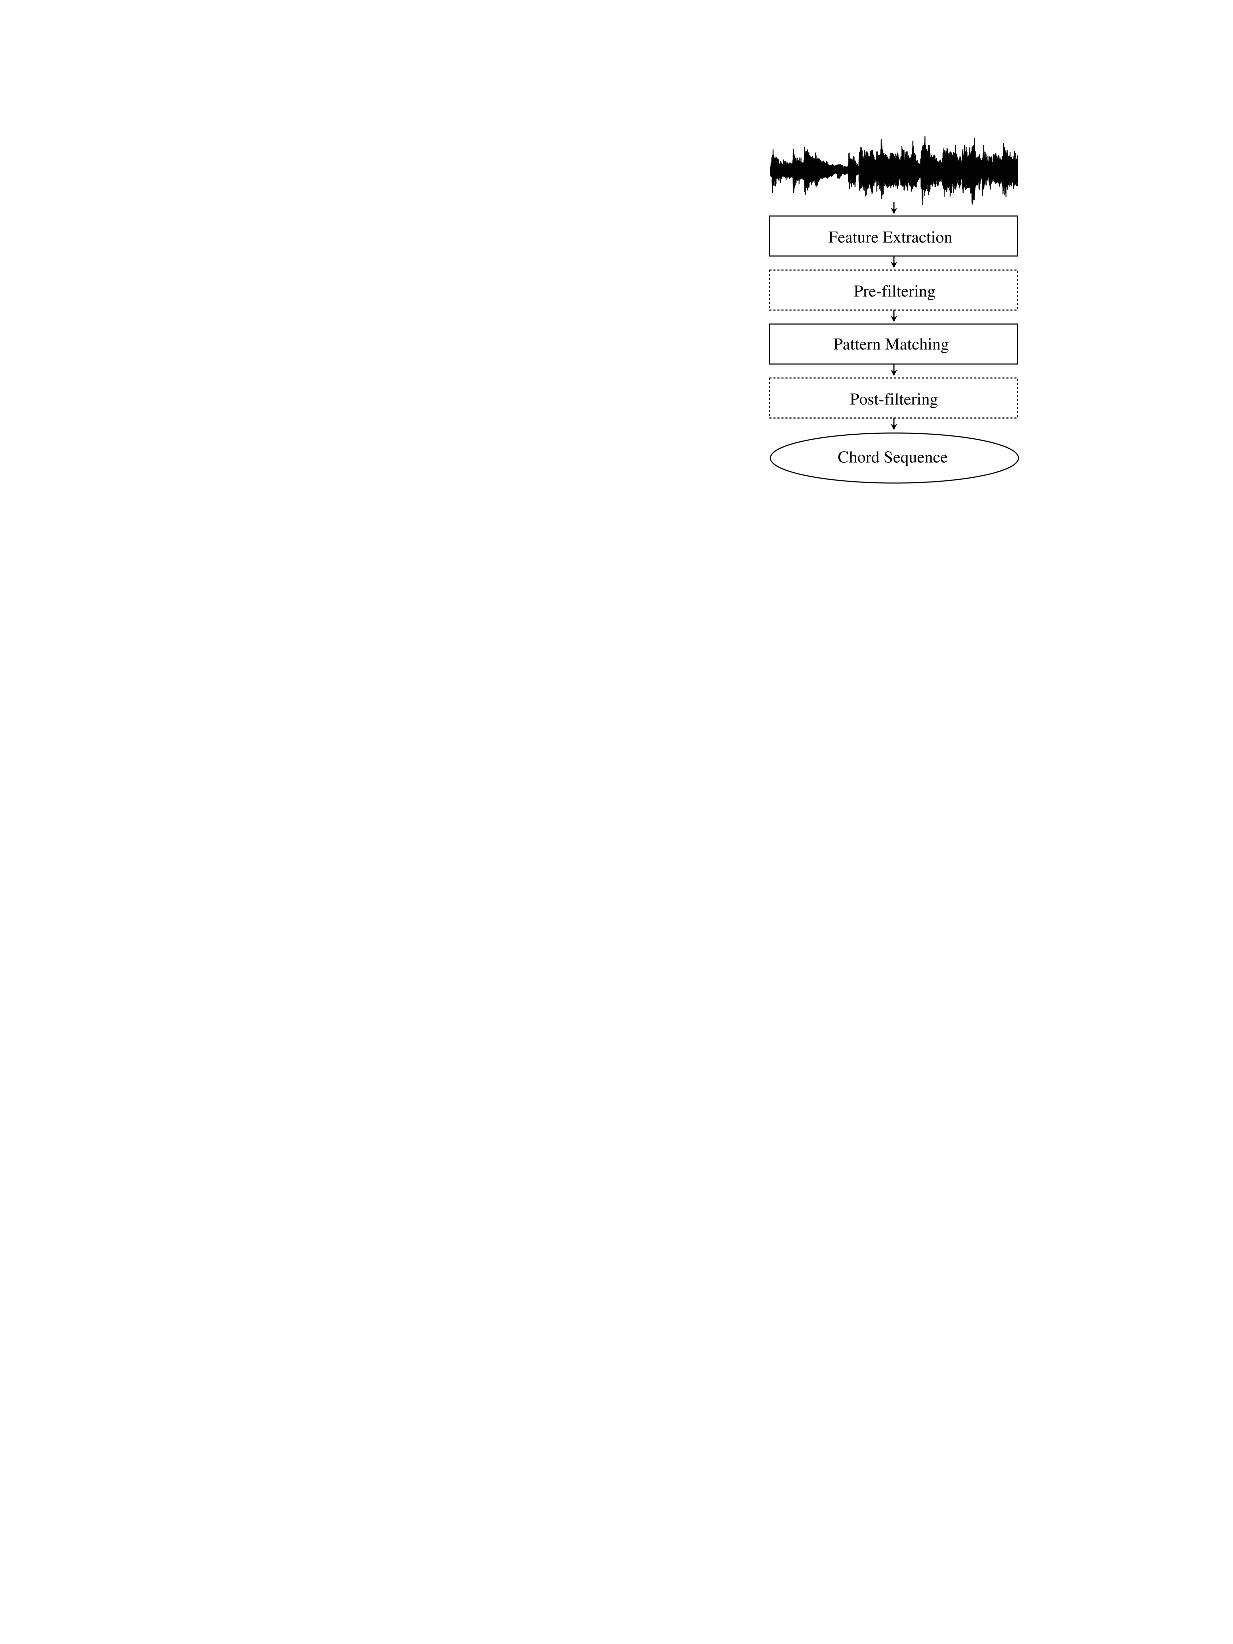
\psfig{file=fig3.pdf,width =3in}
\caption{General layout of the chord recognition system used in~\cite{TaeMin:2014}.}
\label{fig:fig3}
\end{figure}

\subsubsection{Datasets}

The dataset consisted of 180 Beatles songs, 20 Queen songs, 20 songs from the RWC (Real World Computing) pop dataset, and 195 songs from the US-Pop dataset. For training, 5-fold cross validation was used with each group having 99 songs selected randomly. For each fold one group is selected and the other four are used for training. Accuracy is represented by the total duration of correct chords out of the total duration of the dataset~\cite{TaeMin:2014}.

In the first experiment, different combinations of feature extraction and pattern matching are compared to show whether or not model complexity affects performance of the system. They also test the effect of different types of chroma features. The second experiment looks at the pre-filtering techniques of moving filters and beat-synchronization. \todo[inline]{Need to define these and provide more here.} The effect of post-filtering experiment compares the use of different stochastic models. The final experiment uses pre- and post-filtering and again looks at moving filters and beat-synchronization.

\todo[inline]{Needs more work}

\subsubsection{Results}

In the first experiment of this case no filtering is applied during the process. This experiment is testing the difference between preprocessing techniques in the feature extraction stage. Results can be seen in table~\ref{tab:tab6}. The binary template is the hand-made chord model, and the rest are GMMs with a number indicating the number of Gaussian components used. We would expect to see higher accuracy with more processing and more Gaussian components used, but this is not the case. The highest error was in distinguishing major and minor chords with the same root, because two of the notes are shared and the third is only a half-step different.

%Re-make this table as comparing the 4 experiments, the highest result, and what was used to obtain it.

\begin{table*}
\centering
\begin{tabular}{|c|c|c|c|c|c|c|c|} \hline
 & Binary Template & GMM-1 & GMM-5 & GMM-10 & GMM-15 & GMM-20 & GMM-25 \\ \hline
Base & 46.95 & 46.46 & 46.26 & 48.10 & 48.39 & 48.74 & 48.77 \\ \hline
Overtone removal 1 & 52.12 & 49.40 & 47.38 & 50.24 & 51.04 & 51.42 & 51.71 \\ \hline
Overtone removal 2 & 54.38 & 54.51 & 50.49 & 50.90 & 51.42 & 52.14 & 51.97 \\ \hline
Timbre Homogenization 1 & 45.18 & 48.24 & 50.44 & 49.34 & 49.36 & 49.06 & 49.35 \\ \hline
Timbre Homogenization 2 & 44.37 & 40.12 & 39.80 & 39.61 & 40.49 & 40.87 & 40.86 \\ \hline
OR1 \& TH1 & 55.51 & \textbf{58.30} & 57.58 & 57.73 & 57.72 & 57.70 & 57.69 \\ \hline
OR1 \& TH2 & 53.24 & 53.83 & 54.66 & 54.67 & 54.00 & 54.03 & 53.55 \\ \hline
OR2 \& TH1 & 55.00 & 56.29 & 53.09 & 53.24 & 53.28 & 53.33 & 53.43 \\ \hline
\end{tabular}
\caption{Average accuracy without filtering (research case 3, experiment 1).}
\label{tab:tab6}
\end{table*}

\todo[inline]{Need to add the results for pre and post filtering experiments.}


\section{Conclusions}

\todo[inline]{Look at the components of the highest performing systems and determine the best techniques used for feature extraction and pattern matching. Discuss the effects of preprocessing during feature extraction and using HMMs to eliminate unlikely sequences. All of the research cases use PCP and preprocessing of some kind. Case 1 and 3 use GMMs. Case 2 and 3 use HMMs.}

\todo[inline]{Talk about some of the issues and pitfalls with these and all chord recognition systems. Including dense recordings, extremely fast chord changes, and other types of chords that are not recognized. There are also chords that can only be determined by their context and chords that can be interpreted in more than one way.}

\subsection{Future Work}

\todo[inline]{Mention study using online chord database. Genre-specific models.}

\section{Acknowledgements}

%\subsection{Math Equations}
%You may want to display math equations in three distinct styles:
%inline, numbered or non-numbered display.  Each of
%the three are discussed in the next sections.

%\subsubsection{Inline (In-text) Equations}
%A formula that appears in the running text is called an
%inline or in-text formula.  It is produced by the
%\textbf{math} environment, which can be
%invoked with the usual \texttt{{\char'134}begin. . .{\char'134}end}
%construction or with the short form \texttt{\$. . .\$}. You
%can use any of the symbols and structures,
%from $\alpha$ to $\omega$, available in
%\LaTeX\cite{Lamport:LaTeX}; this section will simply show a
%few examples of in-text equations in context. Notice how
%this equation: \begin{math}\lim_{n\rightarrow \infty}x=0\end{math},
%set here in in-line math style, looks slightly different when
%set in display style.  (See next section).
%
%\subsubsection{Display Equations}
%A numbered display equation -- one set off by vertical space
%from the text and centered horizontally -- is produced
%by the \textbf{equation} environment. An unnumbered display
%equation is produced by the \textbf{displaymath} environment.
%
%Again, in either environment, you can use any of the symbols
%and structures available in \LaTeX; this section will just
%give a couple of examples of display equations in context.
%First, consider the equation, shown as an inline equation above:
%%%%%
%\begin{equation*}
%\lim_{n\rightarrow \infty}x=0
%\end{equation*}
%%%%%
%Notice how it is formatted somewhat differently in
%the \textbf{displaymath}
%environment.  Now, we'll enter an unnumbered equation:
%\begin{displaymath}\sum_{i=0}^{\infty} x + 1\end{displaymath}
%and follow it with another numbered equation:
%\begin{equation}\sum_{i=0}^{\infty}x_i=\int_{0}^{\pi+2} f\end{equation}
%just to demonstrate \LaTeX's able handling of numbering.
%
%\subsection{Multi-line formulas}
%%%%%%% \[ \] denotes math; array environment is needed for multi-line
%%%%%%% format, {c} means that the array has one column, centered 
%%%%%%  (alternatives are {l} for left-aligned, {r} for right-aligned)
%%%%%%  \\ denotes a new line
%\[
%\begin{array}{c}
%n_1 = \sum_{i = 1}^k a_i \\
%n_2 = \prod_{i = 1}^k b_i
%\end{array}
%\]
%
%\subsection{Citations}
%Citations to articles \cite{Morman:2006,Lee:2006,TaeMin:2014} listed
%in the Bibliography section of your
%article will occur throughout the text of your article.
%You should use BibTeX to automatically produce this bibliography;
%you simply need to insert one of several citation commands with
%a key of the item cited in the proper location in
%the \texttt{.tex} file \cite{OM:2008}.
%The key is a short reference you invent to uniquely
%identify each work; in this sample document, the key is
%the first author's surname and a
%word from the title.  This identifying key is included
%with each item in the \texttt{.bib} file for your article.
%
%The details of the construction of the \texttt{.bib} file
%are beyond the scope of this sample document, but more
%information can be found in the \textit{Author's Guide},
%and exhaustive details in the \textit{\LaTeX\ User's
%Guide}.
%
%This article shows only the plainest form
%of the citation command, using \texttt{{\char'134}cite}.
%This is what is stipulated in the SIGS style specifications.
%No other citation format is endorsed or supported.
%
%\subsection{Tables}
%Because tables cannot be split across pages, the best
%placement for them is typically the top of the page
%nearest their initial cite.  To
%ensure this proper ``floating'' placement of tables, use the
%environment \textbf{table} to enclose the table's contents and
%the table caption.  The contents of the table itself must go
%in the \textbf{tabular} environment, to
%be aligned properly in rows and columns, with the desired
%horizontal and vertical rules.  Again, detailed instructions
%on \textbf{tabular} material
%is found in the \textit{\LaTeX\ User's Guide}.
%
%Immediately following this sentence is the point at which
%Table 1 is included in the input file; compare the
%placement of the table here with the table in the printed
%dvi output of this document.
%
%\begin{table}
%\centering
%\caption{Frequency of Special Characters}
%\begin{tabular}{|c|c|l|} \hline
%Non-English or Math&Frequency&Comments\\ \hline
%\O & 1 in 1,000& For Swedish names\\ \hline
%$\pi$ & 1 in 5& Common in math\\ \hline
%\$ & 4 in 5 & Used in business\\ \hline
%$\Psi^2_1$ & 1 in 40,000& Unexplained usage\\
%\hline\end{tabular}
%\end{table}
%
%To set a wider table, which takes up the whole width of
%the page's live area, use the environment
%\textbf{table*} to enclose the table's contents and
%the table caption.  As with a single-column table, this wide
%table will ``float" to a location deemed more desirable.
%Immediately following this sentence is the point at which
%Table 2 is included in the input file; again, it is
%instructive to compare the placement of the
%table here with the table in the printed dvi
%output of this document.
%
%
%\begin{table*}
%\centering
%\caption{Some Typical Commands}
%\begin{tabular}{|c|c|l|} \hline
%Command&A Number&Comments\\ \hline
%\texttt{{\char'134}alignauthor} & 100& Author alignment\\ \hline
%\texttt{{\char'134}numberofauthors}& 200& Author enumeration\\ \hline
%\texttt{{\char'134}table}& 300 & For tables\\ \hline
%\texttt{{\char'134}table*}& 400& For wider tables\\ \hline\end{tabular}
%\end{table*}
%% end the environment with {table*}, NOTE not {table}!
%
%\subsection{Figures}
%Like tables, figures cannot be split across pages; the
%best placement for them
%is typically the top or the bottom of the page nearest
%their initial cite.  To ensure this proper ``floating'' placement
%of figures, use the environment
%\textbf{figure} to enclose the figure and its caption.
%
%This sample document contains examples of %\textbf{.eps}
%%and 
%a \textbf{.pdf} file to be displayable with \LaTeX.  More
%details on each of these is found in the \textit{Author's Guide}.
%
%\begin{figure}
%\centering
%\psfig{file=sample_graph.pdf,width =3in}
%\caption{A sample graph just spanning one column.}
%\end{figure}
%
%
%As was the case with tables, you may want a figure
%that spans two columns.  To do this, and still to
%ensure proper ``floating'' placement of tables, use the environment
%\textbf{figure*} to enclose the figure and its caption.
%\begin{figure*}
%\centering
%\psfig{file=sample_graph.pdf,width =5.3in}
%\caption{A sample graph that needs to span two columns of text.}
%\end{figure*}
%and don't forget to end the environment with
%{figure*}, not {figure}!
%
%It's easiest and you tend to get the best quality if your figures vector graphics
%in PDF format. You can include other formats such as PNG, but they will usually
%not look nearly as professional, especially when printed on high resolution printers.
%\emph{Be vary wary of screen captures from other papers. They tend to look pixelated
%and amateurish even at high resolutions.}
%
%\subsection{Theorem-like Constructs}
%Other common constructs that may occur in your article are
%the forms for logical constructs like theorems, axioms,
%corollaries and proofs.  There are
%two forms, one produced by the
%command \texttt{{\char'134}newtheorem} and the
%other by the command \texttt{{\char'134}newdef}; perhaps
%the clearest and easiest way to distinguish them is
%to compare the two in the output of this sample document:
%
%This uses the \textbf{theorem} environment, created by
%the\linebreak\texttt{{\char'134}newtheorem} command:
%\newtheorem{theorem}{Theorem}
%\begin{theorem}
%Let $f$ be continuous on $[a,b]$.  If $G$ is
%an antiderivative for $f$ on $[a,b]$, then
%\begin{displaymath}\int^b_af(t)dt = G(b) - G(a).\end{displaymath}
%\end{theorem}
%
%The other uses the \textbf{definition} environment, created
%by the \texttt{{\char'134}newdef} command:
%\newdef{definition}{Definition}
%\begin{definition}
%If $z$ is irrational, then by $e^z$ we mean the
%unique number which has
%logarithm $z$: \begin{displaymath}{\log e^z = z}\end{displaymath}
%\end{definition}
%
%Two lists of constructs that use one of these
%forms is given in the
%\textit{Author's  Guidelines}.
% 
%There is one other similar construct environment, which is
%already set up
%for you; i.e. you must \textit{not} use
%a \texttt{{\char'134}newdef} command to
%create it: the \textbf{proof} environment.  Here
%is a example of its use:
%\begin{proof}
%Suppose on the contrary there exists a real number $L$ such that
%\begin{displaymath}
%\lim_{x\rightarrow\infty} \frac{f(x)}{g(x)} = L.
%\end{displaymath}
%Then
%\begin{displaymath}
%l=\lim_{x\rightarrow c} f(x)
%= \lim_{x\rightarrow c}
%\left[ g{x} \cdot \frac{f(x)}{g(x)} \right ]
%= \lim_{x\rightarrow c} g(x) \cdot \lim_{x\rightarrow c}
%\frac{f(x)}{g(x)} = 0\cdot L = 0,
%\end{displaymath}
%which contradicts our assumption that $l\neq 0$.
%\end{proof}
%
%Complete rules about using these environments and using the
%two different creation commands are in the
%\textit{Author's Guide}; please consult it for more
%detailed instructions.  If you need to use another construct,
%not listed therein, which you want to have the same
%formatting as the Theorem
%or the Definition\cite{salas:calculus} shown above,
%use the \texttt{{\char'134}newtheorem} or the
%\texttt{{\char'134}newdef} command,
%respectively, to create it.
%
%\subsection*{A {\secit Caveat} for the \TeX\ Expert}
%Because you have just been given permission to
%use the \texttt{{\char'134}newdef} command to create a
%new form, you might think you can
%use \TeX's \texttt{{\char'134}def} to create a
%new command: \textit{Please refrain from doing this!}
%Remember that your \LaTeX\ source code is primarily intended
%to create camera-ready copy, but may be converted
%to other forms -- e.g. HTML. If you inadvertently omit
%some or all of the \texttt{{\char'134}def}s recompilation will
%be, to say the least, problematic.
%
%\section{Conclusions}
%This paragraph will end the body of this sample document.
%Remember that you might still have Acknowledgments or
%Appendices; brief samples of these
%follow.  There is still the Bibliography to deal with; and
%we will make a disclaimer about that here: with the exception
%of the reference to the \LaTeX\ book, the citations in
%this paper are to articles which have nothing to
%do with the present subject and are used as
%examples only.
%
%\section{Acknowledgments}
%
%This section is optional; it is a location for you
%to acknowledge grants, funding, editing assistance and
%what have you.
%
%It is common (but by no means necessary) for students to thank
%their advisor, and possibly other faculty, friends, and family who provided
%useful feedback on the paper as it was being written.
%
%In the present case, for example, the
%authors would like to thank Gerald Murray of ACM for
%his help in codifying this \textit{Author's Guide}
%and the \textbf{.cls} and \textbf{.tex} files that it describes.

% The following two commands are all you need in the
% initial runs of your .tex file to
% produce the bibliography for the citations in your paper.
\bibliographystyle{abbrv}
% sample_paper.bib is the name of the BibTex file containing the
% bibliography entries. Note that you *don't* include the .bib ending here.
\bibliography{sample_paper}  
% You must have a proper ".bib" file
%  and remember to run:
% latex bibtex latex latex
% to resolve all references

\end{document}
